\documentclass[12pt, oneside]{article}

\usepackage[letterpaper, scale=0.8, centering]{geometry}
\usepackage{fancyhdr}
\setlength{\parindent}{0em}
\setlength{\parskip}{1em}

\pagestyle{fancy}
\fancyhf{}
\renewcommand{\headrulewidth}{0pt}
\rfoot{{\footnotesize Copyright Mia Minnes, 2022, Version \today~(\thepage)}}

\author{CSE105Sp22}

\newcommand{\instructions}{{\bf For all HW assignments:}

Weekly homework may be done individually or in groups of up to 3 students. 
You may switch HW partners for different HW assignments. 
The lowest HW score will not be included in your overall HW average. 
Please ensure your name(s) and PID(s) are clearly visible on the first page of your homework submission 
and then upload the PDF to Gradescope. If working in a group, submit only one submission per group: 
one partner uploads the submission through their Gradescope account and then adds the other group member(s) 
to the Gradescope submission by selecting their name(s) in the ``Add Group Members" dialog box. 
You will need to re-add your group member(s) every time you resubmit a new version of your assignment.
 Each homework question will be graded either for correctness (including clear and precise explanations and 
 justifications of all answers) or fair effort completeness. You may only collaborate on HW with CSE 105 students 
 in your group; if your group has questions about a HW problem, you may ask in drop-in help hours or post a private 
 post (visible only to the Instructors) on Piazza.

All submitted homework for this class must be typed. 
You can use a word processing editor if you like (Microsoft Word, Open Office, Notepad, Vim, Google Docs, etc.) 
but you might find it useful to take this opportunity to learn LaTeX. 
LaTeX is a markup language used widely in computer science and mathematics. 
The homework assignments are typed using LaTeX and you can use the source files 
as templates for typesetting your solutions.
To generate state diagrams of machines, we recommend using Flap.js
or JFLAP. Photographs of clearly hand-drawn diagrams may also be used. We recommend that you
submit early drafts to Gradescope so that in case of any technical difficulties, at least some of your
work is present. You may update your submission as many times as you'd like up to the deadline.


{\bf Integrity reminders}
\begin{itemize}
\item Problems should be solved together, not divided up between the partners. The homework is
designed to give you practice with the main concepts and techniques of the course, 
while getting to know and learn from your classmates.
\item You may not collaborate on homework with anyone other than your group members.
You may ask questions about the homework in office hours (of the instructor, TAs, and/or tutors) and 
on Piazza (as private notes viewable only to the Instructors).  
You \emph{cannot} use any online resources about the course content other than the class material 
from this quarter -- this is primarily to ensure that we all use consistent notation and
definitions we will use this quarter and also to protect the learning experience you will have when
the `aha' moments of solving the problem authentically happen.
\item Do not share written solutions or partial solutions for homework with 
other students in the class who are not in your group. Doing so would dilute their learning 
experience and detract from their success in the class.
\end{itemize}

}
\usepackage{amssymb,amsmath,pifont,amsfonts,comment,enumerate,enumitem}
\usepackage{currfile,xstring,hyperref,tabularx,graphicx,wasysym}
\usepackage[labelformat=empty]{caption}
\usepackage[dvipsnames,table]{xcolor}
\usepackage{multicol,multirow,array,listings,tabularx,lastpage,textcomp,booktabs}

\lstnewenvironment{algorithm}[1][] {   
    \lstset{ mathescape=true,
        frame=tB,
        numbers=left, 
        numberstyle=\tiny,
        basicstyle=\rmfamily\scriptsize, 
        keywordstyle=\color{black}\bfseries,
        keywords={,procedure, div, for, to, input, output, return, datatype, function, in, if, else, foreach, while, begin, end, }
        numbers=left,
        xleftmargin=.04\textwidth,
        #1
    }
}
{}
\lstnewenvironment{java}[1][]
{   
    \lstset{
        language=java,
        mathescape=true,
        frame=tB,
        numbers=left, 
        numberstyle=\tiny,
        basicstyle=\ttfamily\scriptsize, 
        keywordstyle=\color{black}\bfseries,
        keywords={, int, double, for, return, if, else, while, }
        numbers=left,
        xleftmargin=.04\textwidth,
        #1
    }
}
{}

\newcommand\abs[1]{\lvert~#1~\rvert}
\newcommand{\st}{\mid}

\newcommand{\A}[0]{\texttt{A}}
\newcommand{\C}[0]{\texttt{C}}
\newcommand{\G}[0]{\texttt{G}}
\newcommand{\U}[0]{\texttt{U}}

\newcommand{\cmark}{\ding{51}}
\newcommand{\xmark}{\ding{55}}
 
 
\title{HW4: Context-free Languages and Turing Machines}
\date{Due: 5/5/22 at 5pm (no penalty late submission until 8am next morning), via Gradescope}

\begin{document}
\maketitle
\thispagestyle{fancy}

{\bf In this assignment,}

You will practice designing and working with context-free grammars and 
pushdown automata. You will use general constructions to explore the class of context-free languages.
You will also practice with the formal definition of Turing machines.

{\bf Resources}: To review the topics you are working with 
for this assignment, see the class material from Weeks 4 and 5.
We will post frequently asked questions and our answers to them in a 
pinned Piazza post.

{\bf Reading and extra practice problems}: Sipser Sections 2.1, 2.2, 2.3 (partially).
Chapter 2 exercises 2.1, 2.2, 2.3, 2.4, 2.6, 2.9, 2.10, 2.11, 2.12, 2.13, 2.16, 2.17. Chapter 2 problem 2.30.
Chapter 3 exercises 3.1, 3.2.

{\bf Key Concepts}: Pushdown automata, stack, context-free grammar, derivations, context-free languages,
Turing machines, halting, looping.

\instructions

You will submit this assignment via Gradescope
(\href{https://www.gradescope.com}{https://www.gradescope.com}) 
in the assignment called ``HW4CSE105Sp22''.

\newpage
{\bf Assigned questions}
\begin{enumerate}
    \item For this question, we are working over the fixed alphabet $\{a,b,c\}$.

    \begin{enumerate}
        \item ({\it Graded for fair effort completeness}\footnote{This means 
        you will get full credit so long as your submission demonstrates honest 
        effort to answer the question. You will not be penalized for incorrect answers. 
        To demonstrate your honest effort in answering the question, we ask that you 
        include your attempt to answer *each* part of the question. If you get stuck 
        with your attempt, you can still demonstrate your effort by explaining where 
        you got stuck and what you did to try to get unstuck.})

    Consider the PDA over this alphabet with state diagram
        \begin{center}
        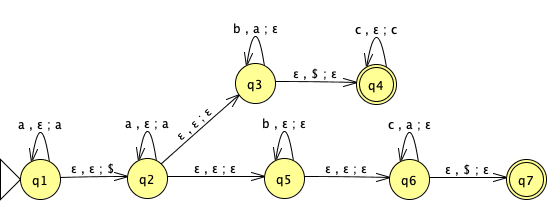
\includegraphics[width=4in]{resources/machines/hw4PDA.png}
        \end{center}

    Give an informal description of this PDA and describe the language it recognizes using 
    set builder notation.

    {\it Hint:} Compare the PDA with the machine in Example 2.16 and Figure 2.17 
    of the textbook (page 116), which recognizes 
    the language $\{a^i b^j c^k \mid i,j,k \geq 0 \textrm{ and } i=j \textrm{ or } i=k\}$ and 
    identify the main differences. 

    \item  ({\it Graded for correctness}\footnote{This means your solution will be
    evaluated not only on the correctness of your answers, but on your ability to 
    present your ideas clearly and logically. You should explain how you arrived at 
    your conclusions, using  mathematically sound reasoning. Whether you use formal proof techniques or 
    write a more informal argument for why 
    something is true, your answers should always be well-supported. Your goal 
    should be to convince the reader that 
    your results and methods are sound.}) 

    Consider the CFG $(\{X, S, S_1, S_2, T, Y\}, \{a,b,c\}, R, X)$ where the set of rules $R$ has
    \begin{align*}
        X &\to aX \mid S \mid T \\
        S &\to S_1S_2 \\
        S_1 &\to aS_1 b \mid \varepsilon \\
        S_2 &\to cS_2 \mid \varepsilon\\
        T &\to aTc \mid Y \\
        Y &\to bT_2 \mid \varepsilon
    \end{align*}

    For each of the following strings, either give a derivation in this grammar that proves the 
    string is in the language generated by the grammar, or explain why there is no such derivation.
    \begin{enumerate}
        \item $aaaa$
        \item $abbc$
        \item $aabb$
    \end{enumerate}
    
    \item ({\it Graded for correctness}) Modify the start variable of this context-free grammar to get a 
    different CFG
    (with the same set of variables, set of terminals, and set of rules)
    that generates an {\bf infinite  regular language}, if possible. A complete solution will include either (1) the 
    formal definition of this new CFG and an explanation of why the language it recognizes
    is both infinite and regular, or (2) a sufficiently general and correct argument for why there is no way to choose 
    the start variable to satisfy this requirement.
    \end{enumerate}

    \item ({\it Graded for correctness}) 
    In this question, you'll practice working with formal general constructions
    for PDAs and translating between state diagrams and formal definitions.

    Suppose 
    \[
    M = (Q, \Sigma, \Gamma, \delta, q_0, F)
    \]
    is a PDA.  We can define a new
PDA $N$ so that $L(M) = L(N)$ and $N$ is {\bf guaranteed to have an empty stack} at the 
end of any accepting computation. 
Informally, the construction is as follows: Add three new states $q_1', q_2', q_3'$ and one new
stack symbol $\#$.  
\begin{itemize}
\item One of the new states $q_1'$ will be the new {\bf start} state and it has a spontaneous transition to the old start state $q_0$ which pushes the new stack symbol $\#$ to the stack. 
\item The transitions between the old states are all the same.
\item From each of the old accept states, {\bf add} a spontaneous
transition (that doesn't modify the stack) to the second new state $q_2'$.  
\item In this state $q_2'$, pop all old stack
symbols from the stack without reading any input. 
\item When the new stack symbol $\#$ is on the top of the stack, transition to the third new state $q_3'$ and accept.
\end{itemize}
Assume $\{ q_1', q_2', q_3'\} \cap Q = \emptyset$ (otherwise, relabel 
some of the states in $Q$) and assume that $\# \notin \Gamma$ (otherwise, relabel this stack symbol 
in $\Gamma$).  Define $N$ to be
\[
N = ( Q \cup \{ q_1', q_2', q_3'\} , \Sigma, \Gamma \cup \{\#\}, \delta_N, q_1', \{q_3'\} )
\]
where 
$\delta_N : Q \cup \{ q_1', q_2', q_3'\}~~\times~~ \Sigma_\varepsilon ~~\times~~\Gamma_\varepsilon\cup \{\#\}
\to \mathcal{P}( Q \cup \{ q_1', q_2', q_3'\} ~~\times ~~\Gamma_\varepsilon\cup \{\#\})$  is defined as
\[
\delta_N ( ~(q, x, y)~) = \begin{cases}
\{ (q_0, \#) \} &\qquad \text{if $q = q_1'$, $x = \varepsilon$, $y = \varepsilon$} \\
\delta( ~(q, x, y)~)  & \qquad \text{if $q \in Q$, $x \in \Sigma$, $y \in \Gamma_\varepsilon$} \\
\delta( ~(q, x, y)~)  & \qquad \text{if $q \in Q$, $x=\varepsilon$, $y \in \Gamma$} \\
\delta( ~(q, x, y)~)  & \qquad \text{if $q \in Q  \setminus F$, $x=\varepsilon$, $y =\varepsilon$} \\
\delta( ~(q, x, y)~) \cup \{  (q_2', \varepsilon) \}  & \qquad \text{if $q \in F$, $x=\varepsilon$, $y =\varepsilon$} \\
\{ (q_2', \varepsilon)\} & \qquad \text{if $q = q_2'$, $x = \varepsilon$, $y \in  \Gamma$} \\
\{ (q_3', \varepsilon)\} & \qquad \text{if $q = q_2'$, $x = \varepsilon$, $y = \#$} \\
\emptyset & \qquad \text{otherwise}
\end{cases}
\]

\begin{enumerate}
\item ({\it Graded for correctness})
Illustrate this construction by considering the PDA $M$ over the input alphabet 
$\{a,b,c\}$
\begin{center}
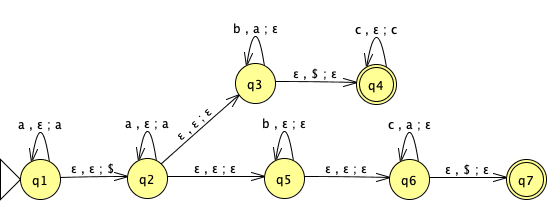
\includegraphics[width=5in]{resources/machines/hw4PDA.png}
\end{center}

and applying the construction above to create the related PDA $N$ and include its state diagram in your submission.
{\it Note: you may include the formal definition of your PDA, but this is not required.} 

\item ({\it Graded for correctness}) Pick a string of length $5$ over the alphabet of the PDA $M$ and use it to demonstrate
the difference in $M$ and in $N$ by 
\begin{itemize}
\item describing an accepting computation of $M$ on this string for which the stack is not empty
at the end of the computation, and
\item describing an accepting computation of $N$ on this string for which the stack is empty at the 
end of the computation.
\end{itemize}
In your descriptions of these computations, include both the sequence of states visited by the machine
as well as snapshots of the full contents of the stack at each step in the computation.  You may hand-draw
and scan these traces of the computations.

{\it Hint}: You will need to pick your example string wisely. It must be accepted by $M$ and 
there must be a computation of $M$ on your string which ends with a nonempty stack. Not all choices
of length $5$ strings work.

\end{enumerate}

\item  ({\it Graded for fair effort completeness})

Fix an arbitrary alphabet $\Sigma$. 
Prove that the class of context-free languages over $\Sigma$ is closed under concatenation in two ways:
\begin{enumerate}
    \item Prove that, for any languages $L_1, L_2$ over $\Sigma$, if there 
    are PDAs $M_1$ and $M_2$ such that $L_1 = L(M_1)$ and $L_2 = L(M_2)$, then there is 
    a PDA that recognizes $L_1 \circ L_2$.
    \item Prove that, for any languages $L_1, L_2$ over $\Sigma$, if there 
    are CFGs $G_1$ and $G_2$ such that $L_1 = L(G_1)$ and $L_2 = L(G_2)$, then there is 
    a CFG that generates $L_1 \circ L_2$.
\end{enumerate}


\item Consider the Turing machine $T$ over the input alphabet $\Sigma = \{0,1\}$ with  the state
    diagram below (the tape alphabet is $\Gamma = \{ 0,1,X,\square\}$).  
    Convention:  any missing transitions in the state diagram have value $(qrej,\square,R)$
    \begin{center}
    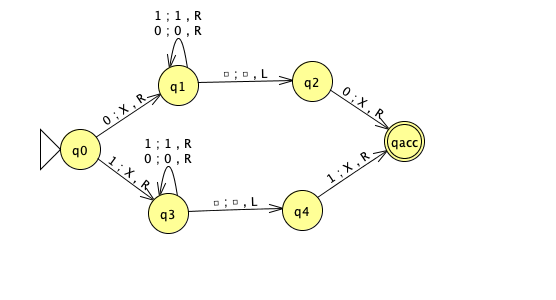
\includegraphics[width=3.5in]{resources/machines/hw4TM.png}
    \end{center}
    \begin{enumerate}

        \item ({\it Graded for correctness}) Specify an example string $w_1$ of length $4$ over 
        $\Sigma$ that is {\bf accepted} by this Turing machine, or explain why there is no such 
        example. A complete solution will include either (1) a precise and clear 
        description of your example  string and a precise and clear description of the accepting computation
        of the Turing machine on this string or (2) a sufficiently
        general and correct argument why there is no such example, referring back to the relevant definitions.
        
        To describe a computation of a Turing machine, include the contents of the 
        tape, the state of the machine, and the location of the read/write head at each step in the computation.
        
        {\it Hint:} In class we've drawn pictures to represent the configuration of the machine at each step 
        in a computation.  You may do so or you may choose to describe these configurations in words.
        
        \item ({\it Graded for correctness}) Specify an example string $w_2$ of length $3$ over $\Sigma$ 
        that is {\bf rejected} by this Turing machine
        or explain why there is no such 
        example. A complete solution will include either (1) a precise and clear 
        description of your example  string and a precise and clear description of the rejecting computation
        of the Turing machine on this string or (2) a sufficiently
        general and correct argument why there is no such example, referring back to the relevant definitions.

        \item ({\it Graded for correctness}) Specify an example string $w_3$ of length $2$ over $\Sigma$ 
        on which  the computation of this Turing machine {\bf loops}
        or explain why there is no such 
        example. A complete solution will include either (1) a precise and clear 
        description of your example  string and a precise and clear description of the looping (non-halting) 
        computation
        of the Turing machine on this string or (2) a sufficiently
        general and correct argument why there is no such example, referring back to the relevant definitions.

        \item ({\it Graded for fair effort completeness}) Write an implementation level description of 
        the Turing machine $T$.
\end{enumerate}

\end{enumerate}
\end{document}